%==============================================================================
\subsection{ Constrained Body Pose }

The geometric-based constraints on acceptable body pose orientations allows the robot to successfully obtain extreme poses without exceeding kienamtic limitations. An example configuration can be seen in Figure \ref{fig:pose_example}.

\begin{figure}[H]
    \centerline{\includegraphics[scale=0.063]{06_results/figures/body_pose_extreme.jpg}}
    \caption{ Example extreme body pose on robot hardware }
    \label{fig:pose_example}
\end{figure}

By dynamically updating the feet workspaces based on the body pose, the robot is able to continue walking without interruptions due to changes in pose configuration. $R_{min}$ and $R_{max}$ also change dynamically as the locations of the workspace centers change. However, as the workspaces shrink, the gait phase occupies less time, resulting in the legs transitioning betweeen stride and support mode faster.

\begin{figure}[H]
    \centerline{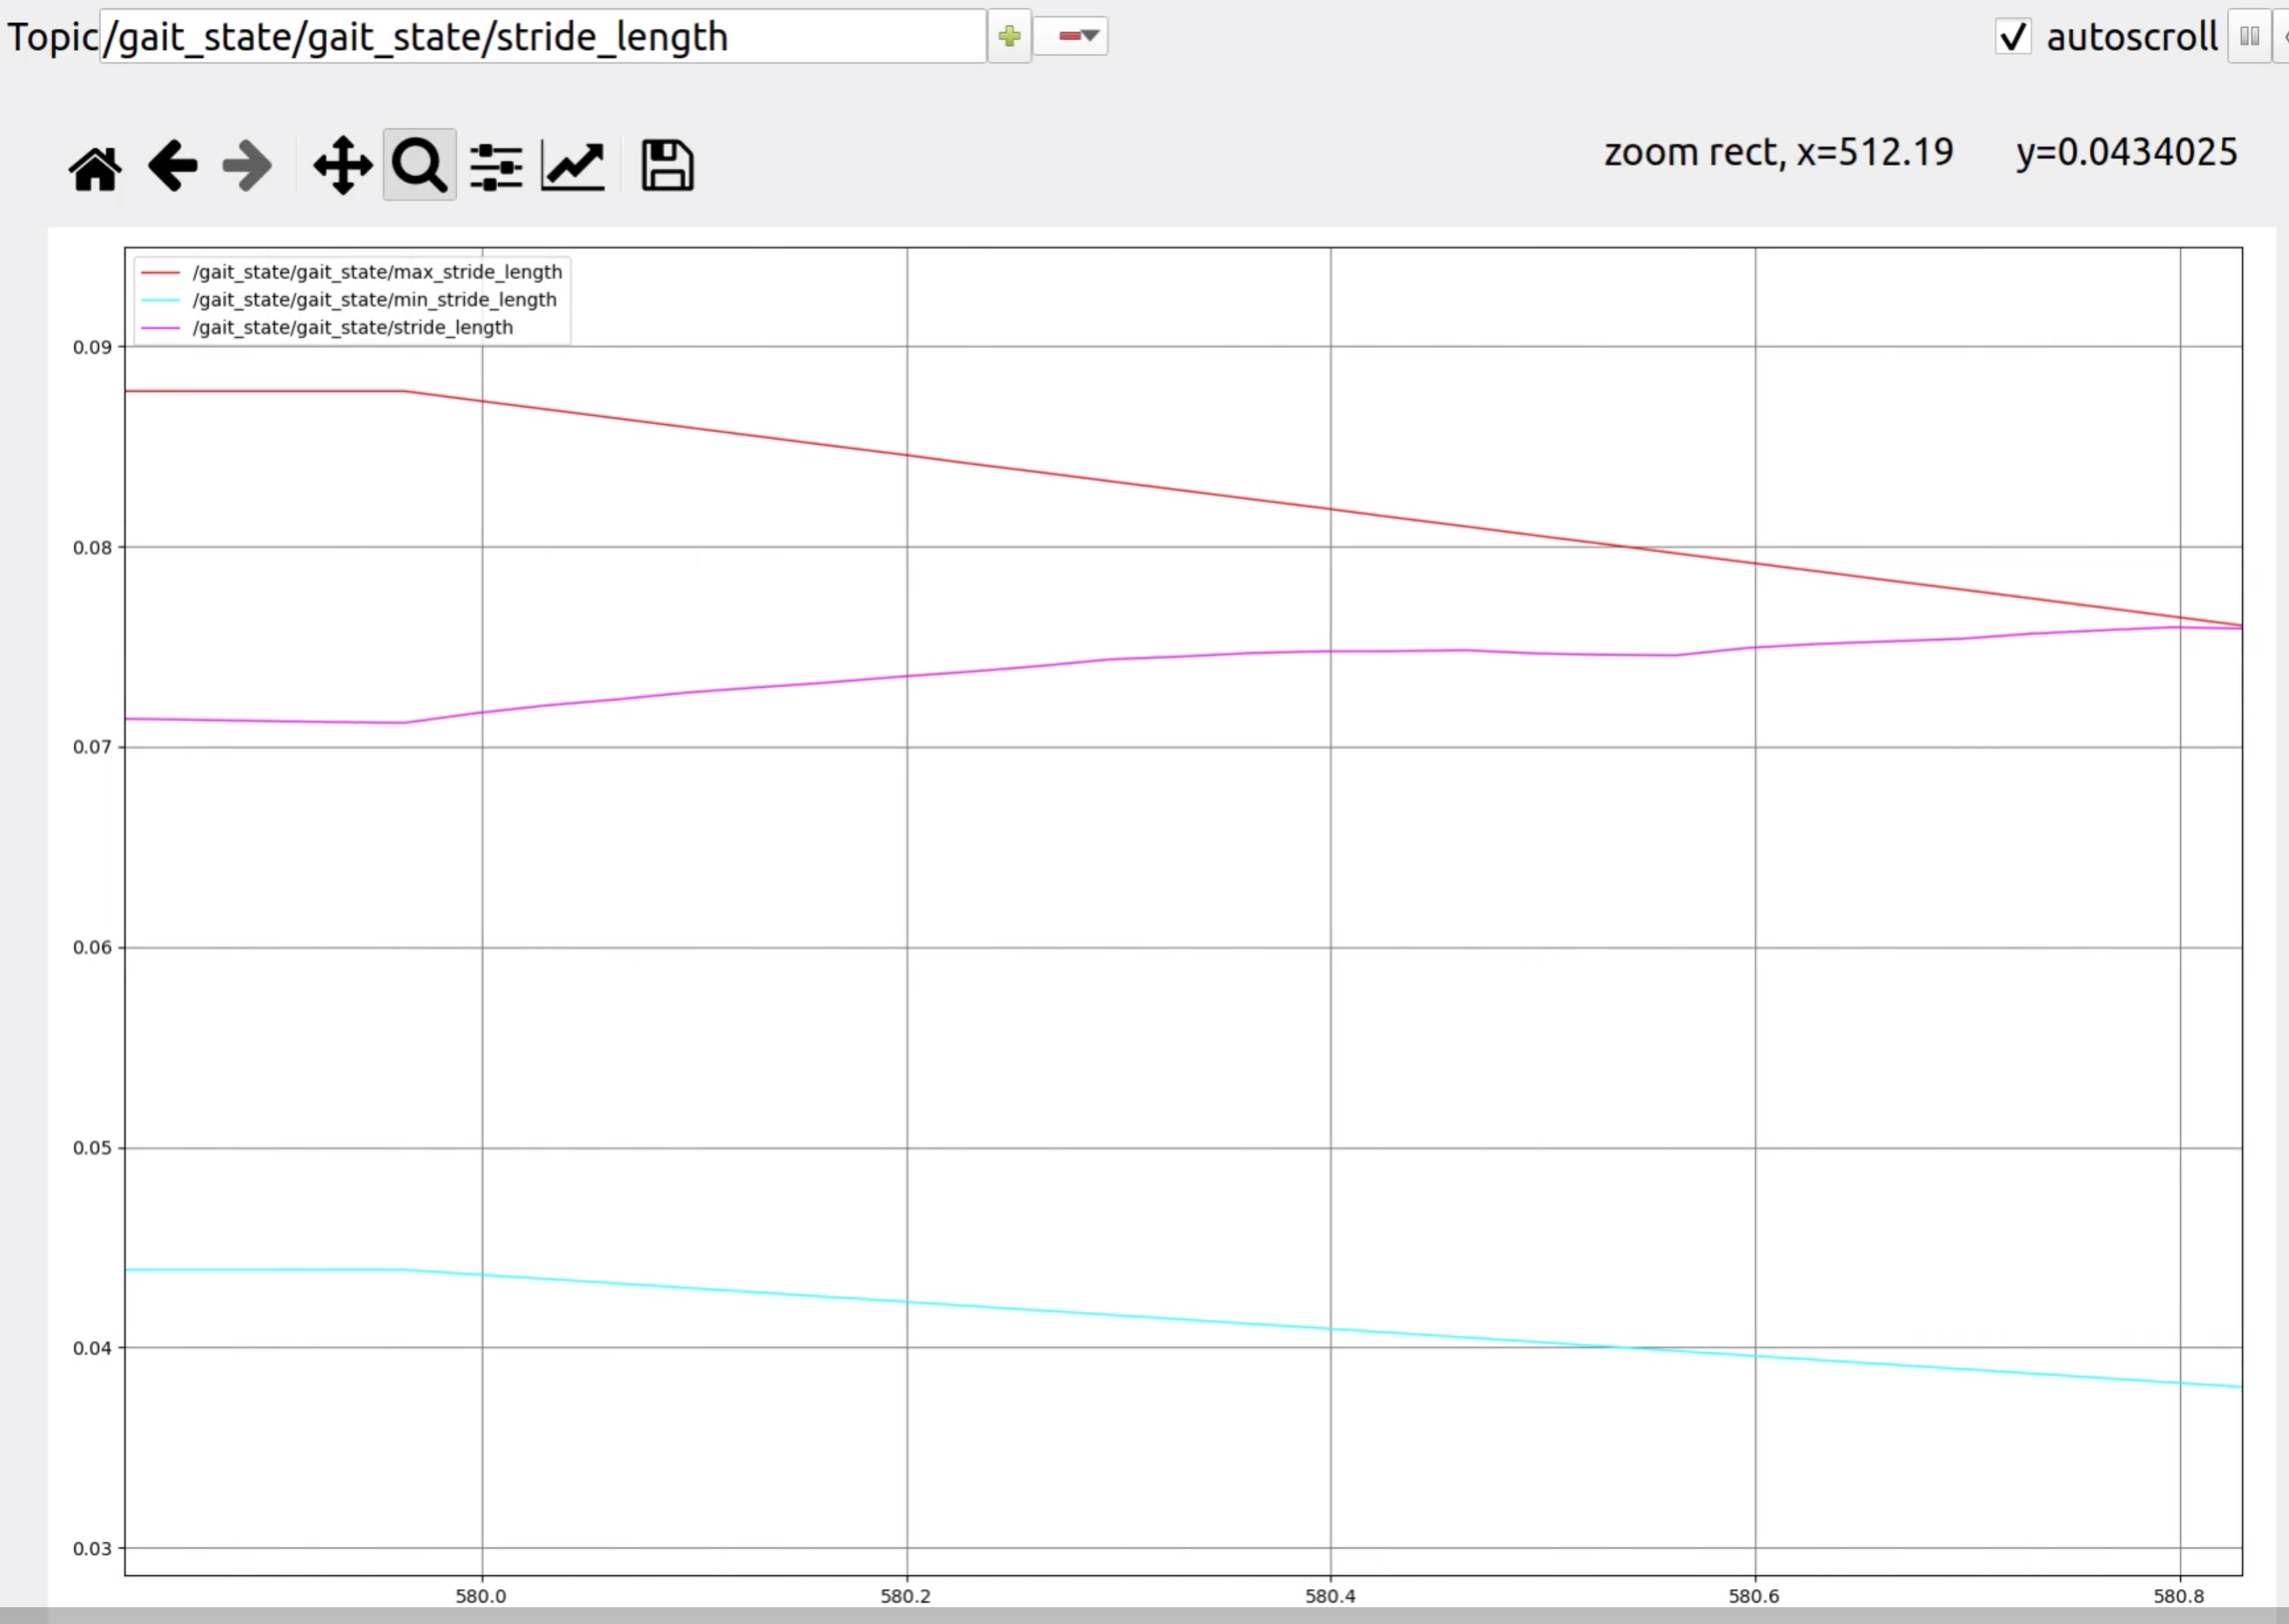
\includegraphics[scale=0.065]{06_results/figures/dynamic_stride_length.png}}
    \caption{ $R_{min}$, $R_{max}$, and $r$ plotted from values on hardware, as the body pose and the workspace centers move }
    \label{fig:dynamic_workspace}
\end{figure}
